\subsection{RQ3: Transfer Across Monitoring Domains}
\label{sec:transfer}




After source-only selection and fitting, the frozen rule transfers between the two development cohorts (Table~\ref{tab:transfer}). RESILIENT$\rightarrow$BrisT1D reaches AUROC $0.735$, and the reverse direction reaches $0.816$, exceeding source history-only scores of $0.698$ and $0.789$, respectively. Within-person scores are $0.571$ and $0.529$.



\paragraph{Transfer of the basis and coefficients.}
We compare target-only fitting, transfer of the source basis, and transfer of both the basis and source coefficients using 22, 43, or 85 Human Rhythms training participants. All conditions use the full HNE extractor, matched participants, and the same regularization candidates. Smaller budgets average three fixed subsets; validation and test participants remain unchanged.

\begin{figure}[H]
\centering
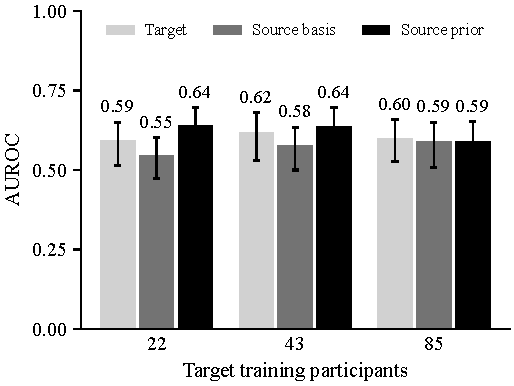
\includegraphics[width=\columnwidth]{figures/human_adaptation.pdf}
\caption{Effect of transferring the source basis and learned coefficients. Intervals jointly resample test participants across conditions and fixed training subsets.}
\label{fig:human-adaptation}
\end{figure}

At 22 participants, the source-coefficient prior reaches mean AUROC $0.639$, compared with $0.593$ for target-only fitting and $0.546$ for basis-only transfer (Figure~\ref{fig:human-adaptation}). Paired gains are $0.046$ (95\% CI: $[0.017,0.077]$) and $0.093$ ($[0.048,0.143]$). The basis-only control retains the source scaling and spline knots; adding the source coefficients supplies the learned link from those coordinates to future risk. This comparison identifies the warning rule itself as useful transferred information. Target-relative gains at 43 and 85 participants are $0.019$ and $-0.011$, respectively; complete budgets appear in Appendix~\ref{app:additional-results}.

\paragraph{Cross-domain endpoints.}
The unchanged extractor and human-source predictor also score industrial faults in CARE and expert-labelled spacecraft events in ESA. Relative to DNB on CARE, AUROC is $0.548$ versus $0.574$; relative to source history on ESA, it is $0.564$ versus $0.498$ on Mission 1 and $0.760$ versus $0.808$ on Mission 2. The Mission 1 gain is $0.066$ (95\% CI: $[-0.018,0.147]$), showing that transfer performance depends on the target domain and endpoint.
